\chapter{Dataset and evaluation metrics}
\label{chap:dataset}
\section{UOT100 Dataset}
Underwater Object Tracking (UOT100) is a benchmark dataset designed to facilitate the development and evaluation of object tracking algorithms specifically tailored for underwater environments \cite{kezebou2019underwater,panetta2021comprehensive}. Unlike traditional tracking datasets that focus on open-air scenarios, UOT100 addresses the unique challenges posed by underwater visual data, including light attenuation, refraction, scattering, and color loss. These distortions significantly impact object visibility and tracking accuracy, making the dataset a crucial resource for advancing research in underwater object tracking.

\begin{figure}
    \centering
    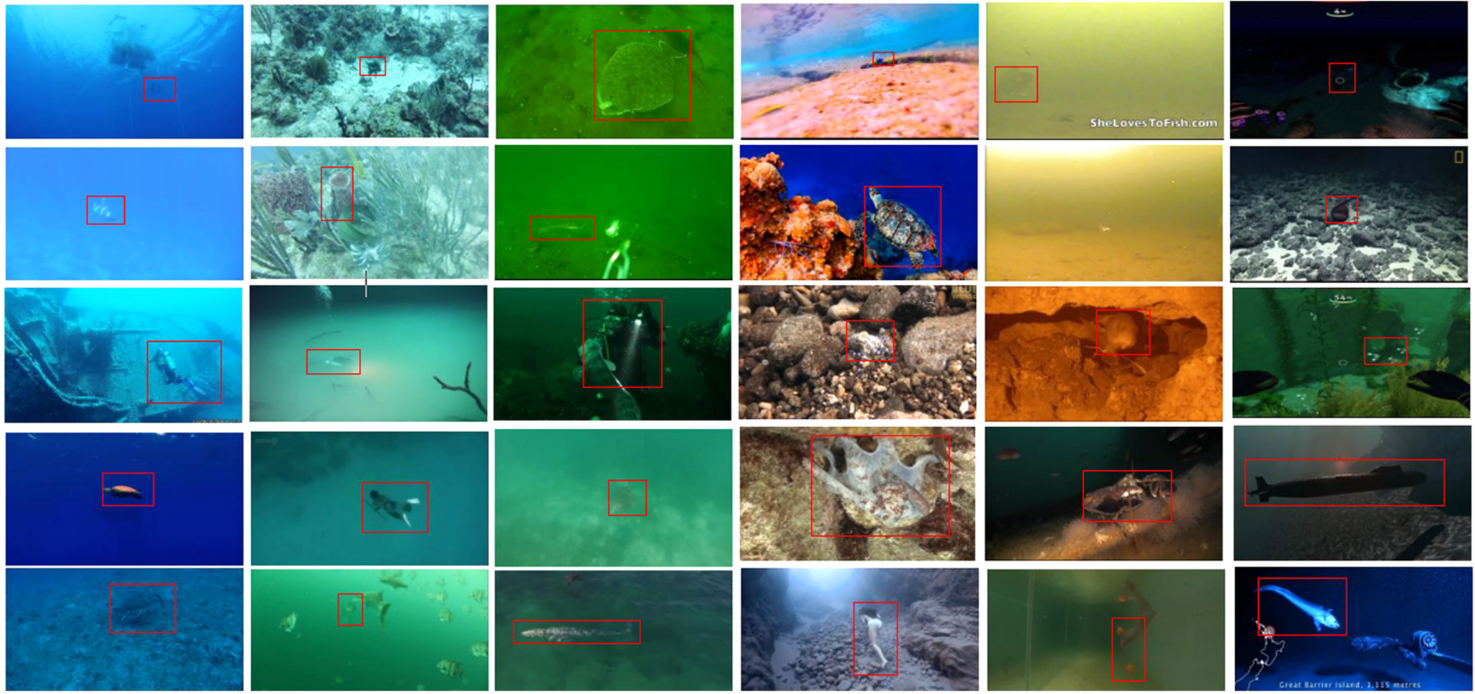
\includegraphics[width=0.8\textwidth]{images/uot100.png}
    \caption{Sample frames from the UOT100 dataset, showcasing various underwater conditions and distortions.}
    \label{fig:uot100_samples}
\end{figure}

The UOT100 dataset consists of 104 video sequences with over 74,000 manually annotated frames. These sequences encompass a diverse range of underwater conditions, including both natural and artificial environments. The dataset includes various types of distortions, such as low contrast, motion blur, occlusions, and fluctuating illumination, which are common in real-world underwater applications.

Each video sequence in the dataset is accompanied by:
\begin{itemize}
    \item An MP4 video file capturing the object of interest.
    \item A ground truth annotation file containing the precise bounding box coordinates for the tracked object.
    \item A description file outlining the distortion types present in the video.
    \item An image sequence folder that stores individual frames for more granular analysis.
\end{itemize}

The dataset is publicly available for research purposes and serves as a standard benchmark for comparing the performance of state-of-the-art tracking algorithms in underwater conditions. It provides a foundation for assessing the robustness of correlation filter-based and deep learning-based tracking methods when applied to challenging aquatic environments



\section{Evaluation Metrics}
To objectively evaluate the performance of object tracking algorithms on the UOT100 dataset, we adopt standard evaluation metrics commonly used in the object tracking community. These metrics include \textbf{Precision}, \textbf{Success Rate (IoU-based evaluation)}, and \textbf{Frames Per Second (FPS)}, which collectively provide a comprehensive assessment of both accuracy and computational efficiency.

\subsection{Precision}
Precision measures the Euclidean distance between the predicted object center and the ground truth center across all frames in a sequence. A prediction is considered accurate if the center distance falls below a given threshold, typically set to 20 pixels as per the One-Pass Evaluation (OPE) protocol \cite{wu2013online}. The precision plot is generated by varying the threshold from 0 to 50 pixels, showing the percentage of frames where the tracker stays within the given error range.

\subsection{Success Rate (IoU-Based Evaluation)}
Success rate is evaluated based on the \textbf{Intersection over Union (IoU)} metric, which quantifies the overlap between the predicted bounding box and the ground truth bounding box. IoU is computed as:

\begin{equation}
IoU = \frac{| B_{pred} \cap B_{gt} |}{| B_{pred} \cup B_{gt} |}
\end{equation}

where $ B_{pred} $ and $ B_{gt} $ represent the predicted and ground truth bounding boxes, respectively. The success rate is derived by counting the number of frames where the IoU exceeds a predefined threshold (e.g., 0.5), and an \textbf{Area Under Curve (AUC)} score is used to rank different tracking algorithms \cite{kristan2018sixth}.

\subsection{Frames Per Second (FPS)}
FPS measures the real-time efficiency of a tracking algorithm by calculating the number of frames processed per second. A higher FPS value indicates a more computationally efficient tracker, which is crucial for real-time underwater applications such as robotic navigation and marine surveillance \cite{nam2016learning}.

By utilizing these metrics, the UOT100 benchmark provides a standardized platform for comparing different tracking approaches and identifying key challenges in underwater object tracking.

\endinput